% Created 2021-03-04 Thu 05:29
% Intended LaTeX compiler: pdflatex
\documentclass[presentation]{beamer}
\usepackage[utf8]{inputenc}
\usepackage[T1]{fontenc}
\usepackage{graphicx}
\usepackage{grffile}
\usepackage{longtable}
\usepackage{wrapfig}
\usepackage{rotating}
\usepackage[normalem]{ulem}
\usepackage{amsmath}
\usepackage{textcomp}
\usepackage{amssymb}
\usepackage{capt-of}
\usepackage{hyperref}
\RequirePackage{fancyvrb}
\DefineVerbatimEnvironment{verbatim}{Verbatim}{fontsize=\scriptsize}
\usetheme{metropolis}
\usecolortheme{}
\usefonttheme{}
\useinnertheme{}
\useoutertheme{}
\author{Petru Rebeja, Marius Apetrii}
\date{4 Martie 2021}
\title{Tehnici Avansate de Programare}
\subtitle{Modularizare, \texttt{git} și evaluare}
\institute[UAIC]{Facultatea de Matematică\\Universitatea Alexandru Ioan Cuza, Iași}
\hypersetup{
 pdfauthor={Petru Rebeja, Marius Apetrii},
 pdftitle={Tehnici Avansate de Programare},
 pdfkeywords={},
 pdfsubject={},
 pdfcreator={Emacs 26.3 (Org mode 9.4.4)},
 pdflang={Romanian}}
\begin{document}

\maketitle
\section{Introducere}
\label{sec:org735d22f}
\begin{frame}[label={sec:org7faad61}]{Informații}
\begin{center}
Avem spațiu dedicat cursului pe Discord.
\end{center}
\begin{center}

\includegraphics[height=0.5\textheight]{img/qr-discord-server.png}
\end{center}
\end{frame}
\begin{frame}[label={sec:org7bdca18},fragile]{Recapitulare}
 \pause
\begin{itemize}
\item Tipuri de date în \texttt{.net}
\end{itemize}
\pause
\begin{itemize}
\item Principiile programării orientată-obiect
\end{itemize}
\end{frame}
\begin{frame}[label={sec:org0698e89}]{Despre ce vom discuta azi}
\begin{itemize}
\item Clase abstracte vs. interfețe.
\item Acuplare și Coeziune.
\item Fluxul de lucru GitHub
\item Evaluare
\end{itemize}
\end{frame}
\section{Clase abstracte vs. Interfețe}
\label{sec:orgcd3e470}
\begin{frame}[label={sec:org04e60d3}]{Clasa abstractă}
\begin{itemize}
\item Oferă o implementare implicită pentru metode și proprietăți.
\item Nu se pot crea instanțe ale claselor abstracte.
\item Este mai puțin abstractă decât înterfața.
\item Poate impune anumite constrângeri (ex. constructorul).
\item Un tip de date poate deriva dintr-o singură clasă abstractă.
\end{itemize}
\end{frame}
\begin{frame}[label={sec:orga57aaf5}]{Interfața}
\begin{itemize}
\item Nu oferă nicio implementare.
\item Cel mai mare grad de abstractizare.
\item Nu impune constrângeri decât asupra semnăturii metodelor.
\item Un tip de date poate implementa mai multe interfețe.
\end{itemize}
\end{frame}
\section{Modularizarea codului-sursă}
\label{sec:org3fab267}
\begin{frame}[label={sec:org57c84b8}]{Acuplare și Coeziune}
Două atribute foarte importante ale unui produs software de succes sunt:
\begin{itemize}
\item Grad mic de acuplare,
\item Grad mare de coeziune.
\end{itemize}
\end{frame}
\begin{frame}[label={sec:orgf9251bb}]{Acuplarea}
\begin{quotation} %% Acuplarea
\alert{Acuplarea} este o măsură a gradului de interdependență dintre modulele unui produs software\footnote{\url{https://en.wikipedia.org/wiki/Coupling\_(computer\_programming)}}.
\end{quotation}
\end{frame}
\begin{frame}[label={sec:orgeb20e74},fragile]{Acuplarea --- exemplu}
 Implementarea clasică a șablonului \texttt{Singleton} este un exemplu de grad înalt de acuplare: clasele care folosesc metodele definite de \texttt{Singleton} sunt dependente de acesta.
\end{frame}
\begin{frame}[label={sec:org14dcba2}]{Coeziunea}
\begin{quotation} %% Coeziunea
\alert{Coeziunea} este măsura în care elementele unui modul aparțin unul de celălalt\footnote{\url{https://en.wikipedia.org/wiki/Cohesion\_(computer\_science)}}.
\end{quotation}
\end{frame}
\section{Fluxul de lucru Git}
\label{sec:org8873567}
\begin{frame}[label={sec:org184972d}]{Git\footnote{\url{https://xkcd.com/1597/}}}
\begin{center}
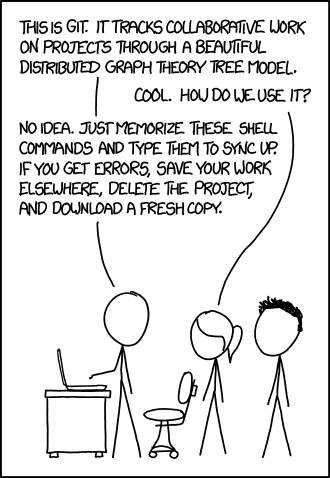
\includegraphics[height=.8\textheight]{img/xkcd-git.png}
\end{center}
\end{frame}
\begin{frame}[label={sec:orgbf03483}]{Fluxul de lucru GitHub\footnote{\url{https://guides.github.com/introduction/flow/}}}
\begin{center}
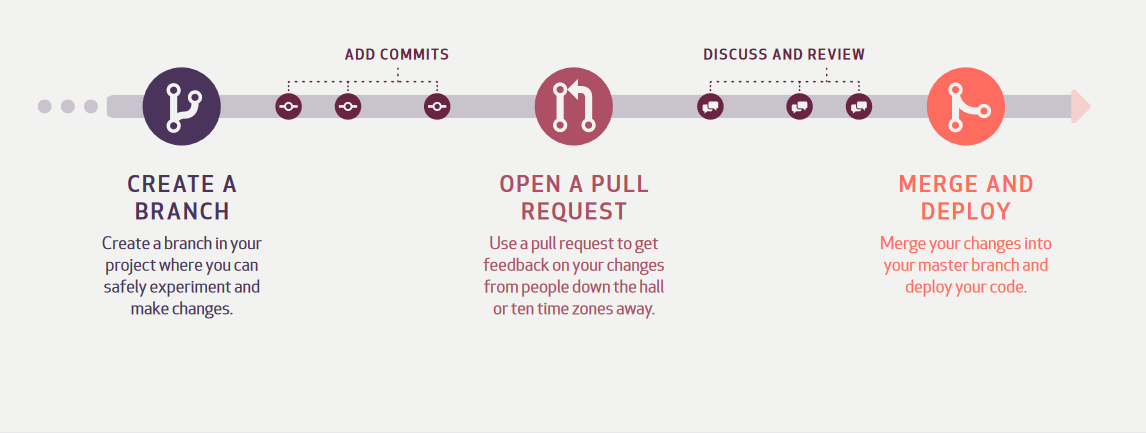
\includegraphics[width=\textwidth]{img/github-flow.png}
\end{center}
\end{frame}
\begin{frame}[label={sec:org8528ceb},fragile]{Fluxul de lucru GitHub}
 Pentru proiectele la care aveți drepturi să faceți modificări:
\begin{itemize}
\item Creați o ramură nouă,
\item Implementați cerințele prin \alert{modificări multiple și atomice},
\item Creați un \alert{Pull Request} din ramura nouă,
\item Revizuiți și modificați dacă este cazul,
\item Îmbinați ramura nouă cu \texttt{main},
\item Livrați funcționalitatea adăugată.
\end{itemize}
\end{frame}
\begin{frame}[label={sec:org1b81611},fragile]{Fluxul de lucru extins\footnote{\url{https://guides.github.com/activities/forking/}}}
 Pentru proiectele la care nu aveți dreptul să faceți modificări:
\begin{itemize}
\item Creați un \texttt{fork} al proiectului,
\item Adăugați modificările necesare în \texttt{fork}-ul propriu (folosing fluxul de lucru de mai sus),
\item Creați un \texttt{Pull Request} din \texttt{fork}-ul propriu,
\item Adăugați modificări suplimentare dacă este cazul
\item O persoană desemnată va decide dacă modificările vor fi acceptate sau nu.
\end{itemize}
\end{frame}
\begin{frame}[label={sec:org7fc7b0b}]{Descrierea modificărilor\footnote{\url{https://xkcd.com/1296/}}}
\begin{center}
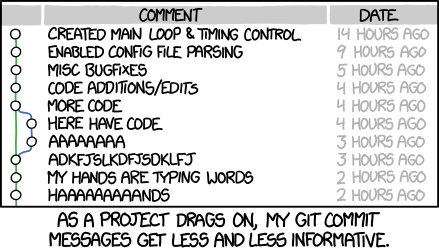
\includegraphics[width=.7\textwidth]{img/xkcd-git-commit.png}
\end{center}
\end{frame}
\begin{frame}[label={sec:org7e975e7}]{Ghid pentru descrierea modificărilor\footnote{\url{https://chris.beams.io/posts/git-commit/}}}
\begin{itemize}
\item Lăsați o linie goală între sumar și restul descrierii.
\item Sumarul trebuie să aibă maxim 50 caractere.
\item Scrieți conform regulilor de gramatică și ortografie:
\begin{itemize}
\item Începeți propozițiile cu majusculă,
\item Nu puneți punct după sumar.
\end{itemize}
\item Descrierea trebuie să explice \alert{ce} și \alert{de ce} a fost modificat; nu \emph{cum}.
\end{itemize}
\end{frame}
\section{Evaluare}
\label{sec:orgfa6717f}
\begin{frame}[label={sec:org8fabe1c}]{Întrebări?}
\begin{center}
Întrebări legate de prima evaluare.
\end{center}
\end{frame}
\section{Încheiere}
\label{sec:org8a0f8ff}
\begin{frame}[label={sec:orgc2a743f}]{Recapitulare}
\begin{itemize}
\item Clase abstracte vs. interfețe.
\item Acuplare și Coeziune.
\item Fluxul de lucru GitHub
\item Evaluare
\end{itemize}
\end{frame}
\begin{frame}[label={sec:org51fa549}]{Vă mulțumesc}
\begin{center}
Succes la evaluare!
\end{center}
\end{frame}
\end{document}